% vim: set textwidth=78 autoindent:

\subsection{Complementes de Ilustraciones}

% when the revision of a section has been finalized, 
% comment out the following line:
% \updatedisclaimer

Los complementos de ilustraciones incluyen el complemento de etiqueta de Copyright, el complemento de Flecha 
de Norte y el complemento de Barra de Escala. Son usados para ``decorar'' el mapa 
agregando elementos cartográficos. 

\subsubsection{Complemento de etiqueta de Copyright}

el título de este complemento es un poco engañoso - puede agregar cualquier texto aleatorio al mapa.

\begin{figure}[ht]
   \begin{center}
   \caption{Complemento de etiqueta de Copyright \nixcaption}\label{fig:copyright}\smallskip
   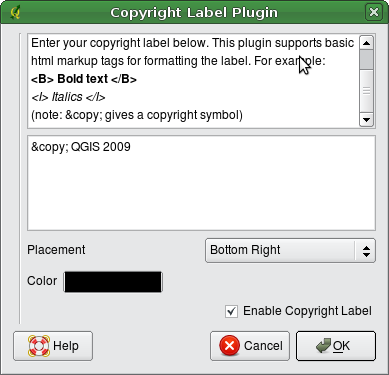
\includegraphics[clip=true, width=8cm]{copyright}
\end{center}  
\end{figure}

\begin{enumerate}
\item Asegúrese  que el complemento está cargado
\item Haga clic en \mainmenuopt{Complementos} > \dropmenuopt{Decoraciones} > \dropmenuopttwo{copyright_label}{Etiqueta de Copyright} o use el botón \toolbtntwo{copyright_label}{Etiqueta de Copyright} de la barra de herramientas.
\item Capture el texto que desee colocar en el mapa. Puede usar HTML como el que se muestra en 
  el ejemplo
\item Elija la posición de la etiqueta desde la caja desplegable \selectstring{Posición}{En la parte inferior derecha}
\item Asegúrese que la caja de selección \checkbox{Activar etiqueta de Copyright} esta activada
\item Clic \button{OK} 
\end{enumerate}

En el ejemplo de arriba (predeterminado) coloca un símbolo de copyright seguido por la fecha en la esquina inferior 
derecha del canvas del mapa.

\subsubsection{Complemento de Flecha de Norte}

El complemento de Flecha de Norte coloca una flecha simple de norte al canvas del mapa. Al
presente hay solo un estilo disponible. Puede ajustar el angulo de la flecha
o permitir que QGIS establezca la dirección automáticamente. Si elije permitir a
QGIS determinar la dirección, este hace su mejor estimación de como la flecha debería de
estar orientada. Para el posicionamiento de la flecha tiene cuatro opciones, 
correspondientes a las cuatro esquinas del canvas del mapa.

\begin{figure}[ht]
   \begin{center}
   \caption{Complemento de Flecha de Norte \nixcaption}\label{fig:north_arrow}\smallskip
   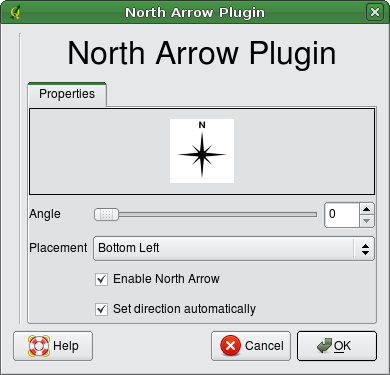
\includegraphics[clip=true, width=8cm]{north_arrow_dialog}
\end{center}  
\end{figure}

\subsubsection{Complemento de Barra de Escala}
El complemento de Barra de Escala agrega una barra de escala simple al canvas del mapa. Usted controla
el estilo y la ubicación, así como el etiquetado de la barra. 

QGIS solo soporta mostrar la escala en las mismas unidades de su marco de mapa. De esta manera
si las unidades de sus capas están en metros, no puede crear una barra de escala en
pies. De la misma manera si está usando grados decimales, no puede crear una barra de escala
que muestre la distancia en metros.

Para agregar una barra de escala:

\begin{enumerate}
\item Clic en \mainmenuopt{Complementos} > \dropmenuopt{Ilustraciones} > \dropmenuopttwo{scale_bar}{Barra de Escala} o use el botón \toolbtntwo{scale_bar}{Barra de Escala} de la barra de herramientas.
\item Elija la posición desde la lista desplegable \selectstring{Ubicación}{Izquierda inferior}
\item Elija el estilo desde  \selectstring{Scale bar style}{Tick Down} list
\item Selecciones el color para la barra \selectcolor{Color de la barra}{negro} o use el color negro predeterminado
\item Establezca el tamaño de la barra y su etiqueta \selectnumber{Tamaño de la barra}{30 grados}
\item Asegúrese de que la caja de verificación \checkbox{Activar barra de escala} está activada
\item Opcionalmente elija redondear un número cuando el canvas cambia de tamaño \checkbox{Redondear números automáticamente al cambiar tamaño}
\item Clic \button{OK} 
\end{enumerate} 

\begin{figure}[ht]
   \begin{center}
   \caption{Scale Bar Plugin \nixcaption}\label{fig:scale_bar}\smallskip
   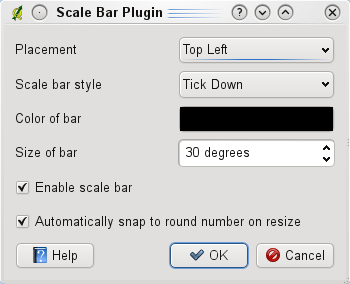
\includegraphics[clip=true, width=8cm]{scale_bar_dialog}
\end{center}  
\end{figure}
